\section{Solution internet : BITTLE}
Bittle est une solution décisionnelle, accesible par le web selon le modèle SaaS (Software as a Service). Bittle permet de construire des tableaux de bord et reporting en ligne grâce au suivi d'indicateurs. On peut donc retrouver l'ensemble des fonctionnalités de cette solution à l'adresse internet suivante :  www.bittle-solutions.com . L'offre qu'elle propose aux entreprise représente un coût de 149 €/mois/utilisateur.
Cette solution permet à l'utilisateur de ne voir que la partie visible du cloud computing (externalisation des serveurs).
\subsection{Fonctionnement de la solution}
\subsubsection{Connexion}
L'utilisateur se connecte à son compte à partir d'un
navigateur (IE, firefox, chrome) via un accès sécurisé.
\begin{figure}[H]
\begin{center}
  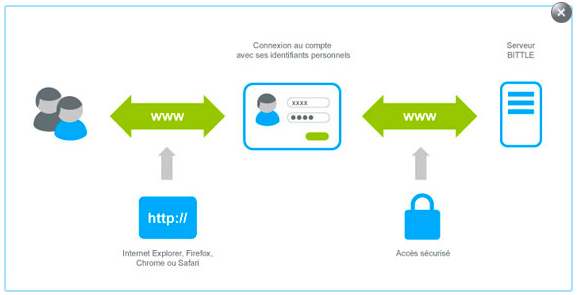
\includegraphics[scale= 0.6]{connexion.png}
  \caption{Protocole de connexion}
\end{center}  
\end{figure}
\subsubsection{Indicateurs}
L'utlisateur doit choisir les indicateurs qu'il souhaite piloter. Il a plusieurs possibilités :
\begin{itemize}
\item[•]L’utilisateur sélectionne les indicateurs parmi la bibliothèque d’indicateurs standard proposée par bittle. L’utilisateur met à disposition ses données brutes afin d’alimenter les indicateurs choisis. La solution bittle établit, de façon automatique, les liens (mapping) entre les données brutes et les indicateurs choisis.
\item[•]L’utilisateur envoie un fichier de données brutes à bittle. Celui-ci est analysé, et les indicateurs de la bibliothèque pouvant être alimentés par ces données sont mis en évidence et proposés à l’utilisateur.
\item[•]Bittle offre également la possibilité de créer ses propres indicateurs. Ainsi, l’utilisateur choisit lui-même les données nécessaires et les règles de calcul correspondantes. 
\end{itemize} 

\begin{figure}[H]
\begin{center}
  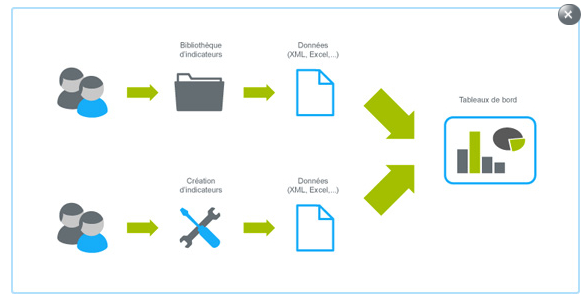
\includegraphics[scale= 0.6]{indicateur.png}
  \caption{Protocole pour le choix d'indicateurs}
\end{center}  
\end{figure}

\subsubsection{Chargement des données}
Le chargement des données pour alimenter les indicateurs de performance sélectionnés peut se faire de plusieurs manières :
\begin{itemize}

\item[•]\textbf{DataAnalyser : } traitement automatique ou manuel des fichiers csv, excel ou xml issus de n’importe quelle application source.

\begin{figure}[H]
\begin{center}
  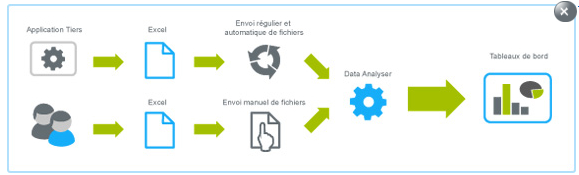
\includegraphics[scale= 0.6]{dataAnalyser.png}
  \caption{Protocole DataAnalyser pour le chargement des données}
\end{center}  
\end{figure}

\item[•]\textbf{DataMailAnalyser : } possibilité d’envoyer des données par email si l’application source dispose de cette fonctionnalité. Le contenu de ce dernier sera ensuite analysé par notre module.

\begin{figure}[H]
\begin{center}
  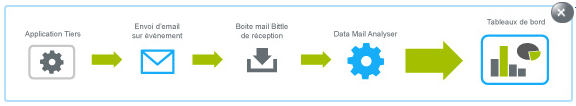
\includegraphics[scale= 0.6]{dataMailAnalyser.png}
  \caption{Protocole DataMailAnalyser pour le chargement des données}
\end{center}  
\end{figure}

\item[•]\textbf{WebAnalyser :}  communication avec des applications tierces via des Web Services.

\begin{figure}[H]
\begin{center}
  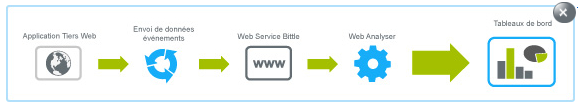
\includegraphics[scale= 0.6]{webAnalyser.png}
  \caption{Protocole WebAnalyser pour le chargement des données}
\end{center}  
\end{figure}

\end{itemize}

\subsubsection{Tableaux de bord, rapport et partage}
Bittle permet de visualiser ses données dans des tableaux de bord, via des indicateurs de performance personnalisables. Ces indicateurs peuvent ensuite être analysés globalement ou en détail, sur une période définie par l’utilisateur. Les tableaux de bord ainsi obtenus peuvent ensuite être partagés, envoyés par email ou exportés pour être intégrés dans une présentation annexe.

\begin{figure}[H]
\begin{center}
  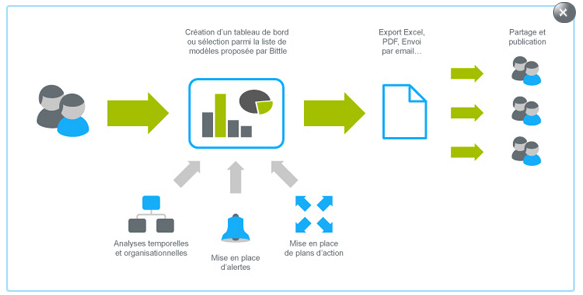
\includegraphics[scale= 0.6]{tableau.png}
  \caption{Protocole pour l'obtention de tableaux de bord}
\end{center}  
\end{figure}

\subsection{Avantages, Inconvénients de la solution}
\subsubsection{Avantages de la solution}
La solution Bittle présentée ci dessus présente de nombreux points forts par rapport aux autres offre du marché :
 
\begin{itemize}
\item[•]Absence de logiciel : cette solution ne nécessite aucune installation de logiciel sur les postes.
\item[•]Accessibilité : comme il s'agit d'une solution web, il est possible d'y accéder partout des lors qu'il y a une connexion internet.
\item[•]Coût : c'est une solution abordable pour les PME car comme annoncé plus haut cette solution coûte environ 150 €/mois/utilisateur.
\item[•]Maintenance : La maintenance du site est transparente pour les utilisateur.
\item[•]Sécurité : Bittle utilise les technologie mise en place par google.
\item[•]Collaboratif : il est possible de partager les données entre plusieurs utilisateurs.
\end{itemize}

\subsubsection{Inconvénients de la solution}

\begin{itemize}
\item[•]Limité : cette solution est limitée car elle permet uniquement de faire du reporting et des tableaux de bords. Bien qu'elle s'étende aux différents coeur de métier d'une entreprise, elle ne permet pas de faire par exemple du data mining.
\item[•] Fiabilité : c'est une solution est peu utiliser actuellement on peut se demander si elle est fiable, de plus elle utilise la technique du cloud computing, elle stock donc les données sur des serveurs externes.
\item[•]Internet : Bittle nécessite une connexion internet
\item[•]Compatibilité: elle n'est pas utilisable sur tout les navigateurs uniquement sur firefox, chrome et internet explorer.
\end{itemize}